\documentclass[11pt,a4paper]{report}
\usepackage[textwidth=37em,vmargin=30mm]{geometry}
\usepackage{calc,xunicode,amsmath,amssymb,paralist,enumitem,tabu,booktabs,datetime2,xeCJK,xeCJKfntef,listings}
\usepackage{tocloft,fancyhdr,tcolorbox,xcolor,graphicx,eso-pic,xltxtra,xelatexemoji}

\newcommand{\envyear}[0]{2025}
\newcommand{\envdatestr}[0]{2025-09-13}
\newcommand{\envfinaldir}[0]{webdb/2025/20250913/final}

\usepackage[hidelinks]{hyperref}
\hypersetup{
    colorlinks=false,
    pdfpagemode=FullScreen,
    pdftitle={Web Digest - \envdatestr}
}

\setlength{\cftbeforechapskip}{10pt}
\renewcommand{\cftchapfont}{\rmfamily\bfseries\large\raggedright}
\setlength{\cftbeforesecskip}{2pt}
\renewcommand{\cftsecfont}{\sffamily\small\raggedright}

\setdefaultleftmargin{2em}{2em}{1em}{1em}{1em}{1em}

\usepackage{xeCJK,xeCJKfntef}
\xeCJKsetup{PunctStyle=plain,RubberPunctSkip=false,CJKglue=\strut\hskip 0pt plus 0.1em minus 0.05em,CJKecglue=\strut\hskip 0.22em plus 0.2em}
\XeTeXlinebreaklocale "zh"
\XeTeXlinebreakskip = 0pt


\setmainfont{Brygada 1918}
\setromanfont{Brygada 1918}
\setsansfont{IBM Plex Sans}
\setmonofont{JetBrains Mono NL}
\setCJKmainfont{Noto Serif CJK SC}
\setCJKromanfont{Noto Serif CJK SC}
\setCJKsansfont{Noto Sans CJK SC}
\setCJKmonofont{Noto Sans CJK SC}

\setlength{\parindent}{0pt}
\setlength{\parskip}{8pt}
\linespread{1.15}

\lstset{
	basicstyle=\ttfamily\footnotesize,
	numbersep=5pt,
	backgroundcolor=\color{black!5},
	showspaces=false,
	showstringspaces=false,
	showtabs=false,
	tabsize=2,
	captionpos=b,
	breaklines=true,
	breakatwhitespace=true,
	breakautoindent=true,
	linewidth=\textwidth
}






\newcommand{\coverpic}[2]{
    % argv: itemurl, authorname
    Cover photo by #2~~(\href{#1}{#1})
}
\newcommand{\makeheader}[0]{
    \begin{titlepage}
        % \newgeometry{hmargin=15mm,tmargin=21mm,bmargin=12mm}
        \begin{center}
            
            \rmfamily\scshape
            \fontspec{BaskervilleF}
            \fontspec{Old Standard}
            \fontsize{59pt}{70pt}\selectfont
            WEB\hfill DIGEST
            
            \vfill
            % \vskip 30pt
            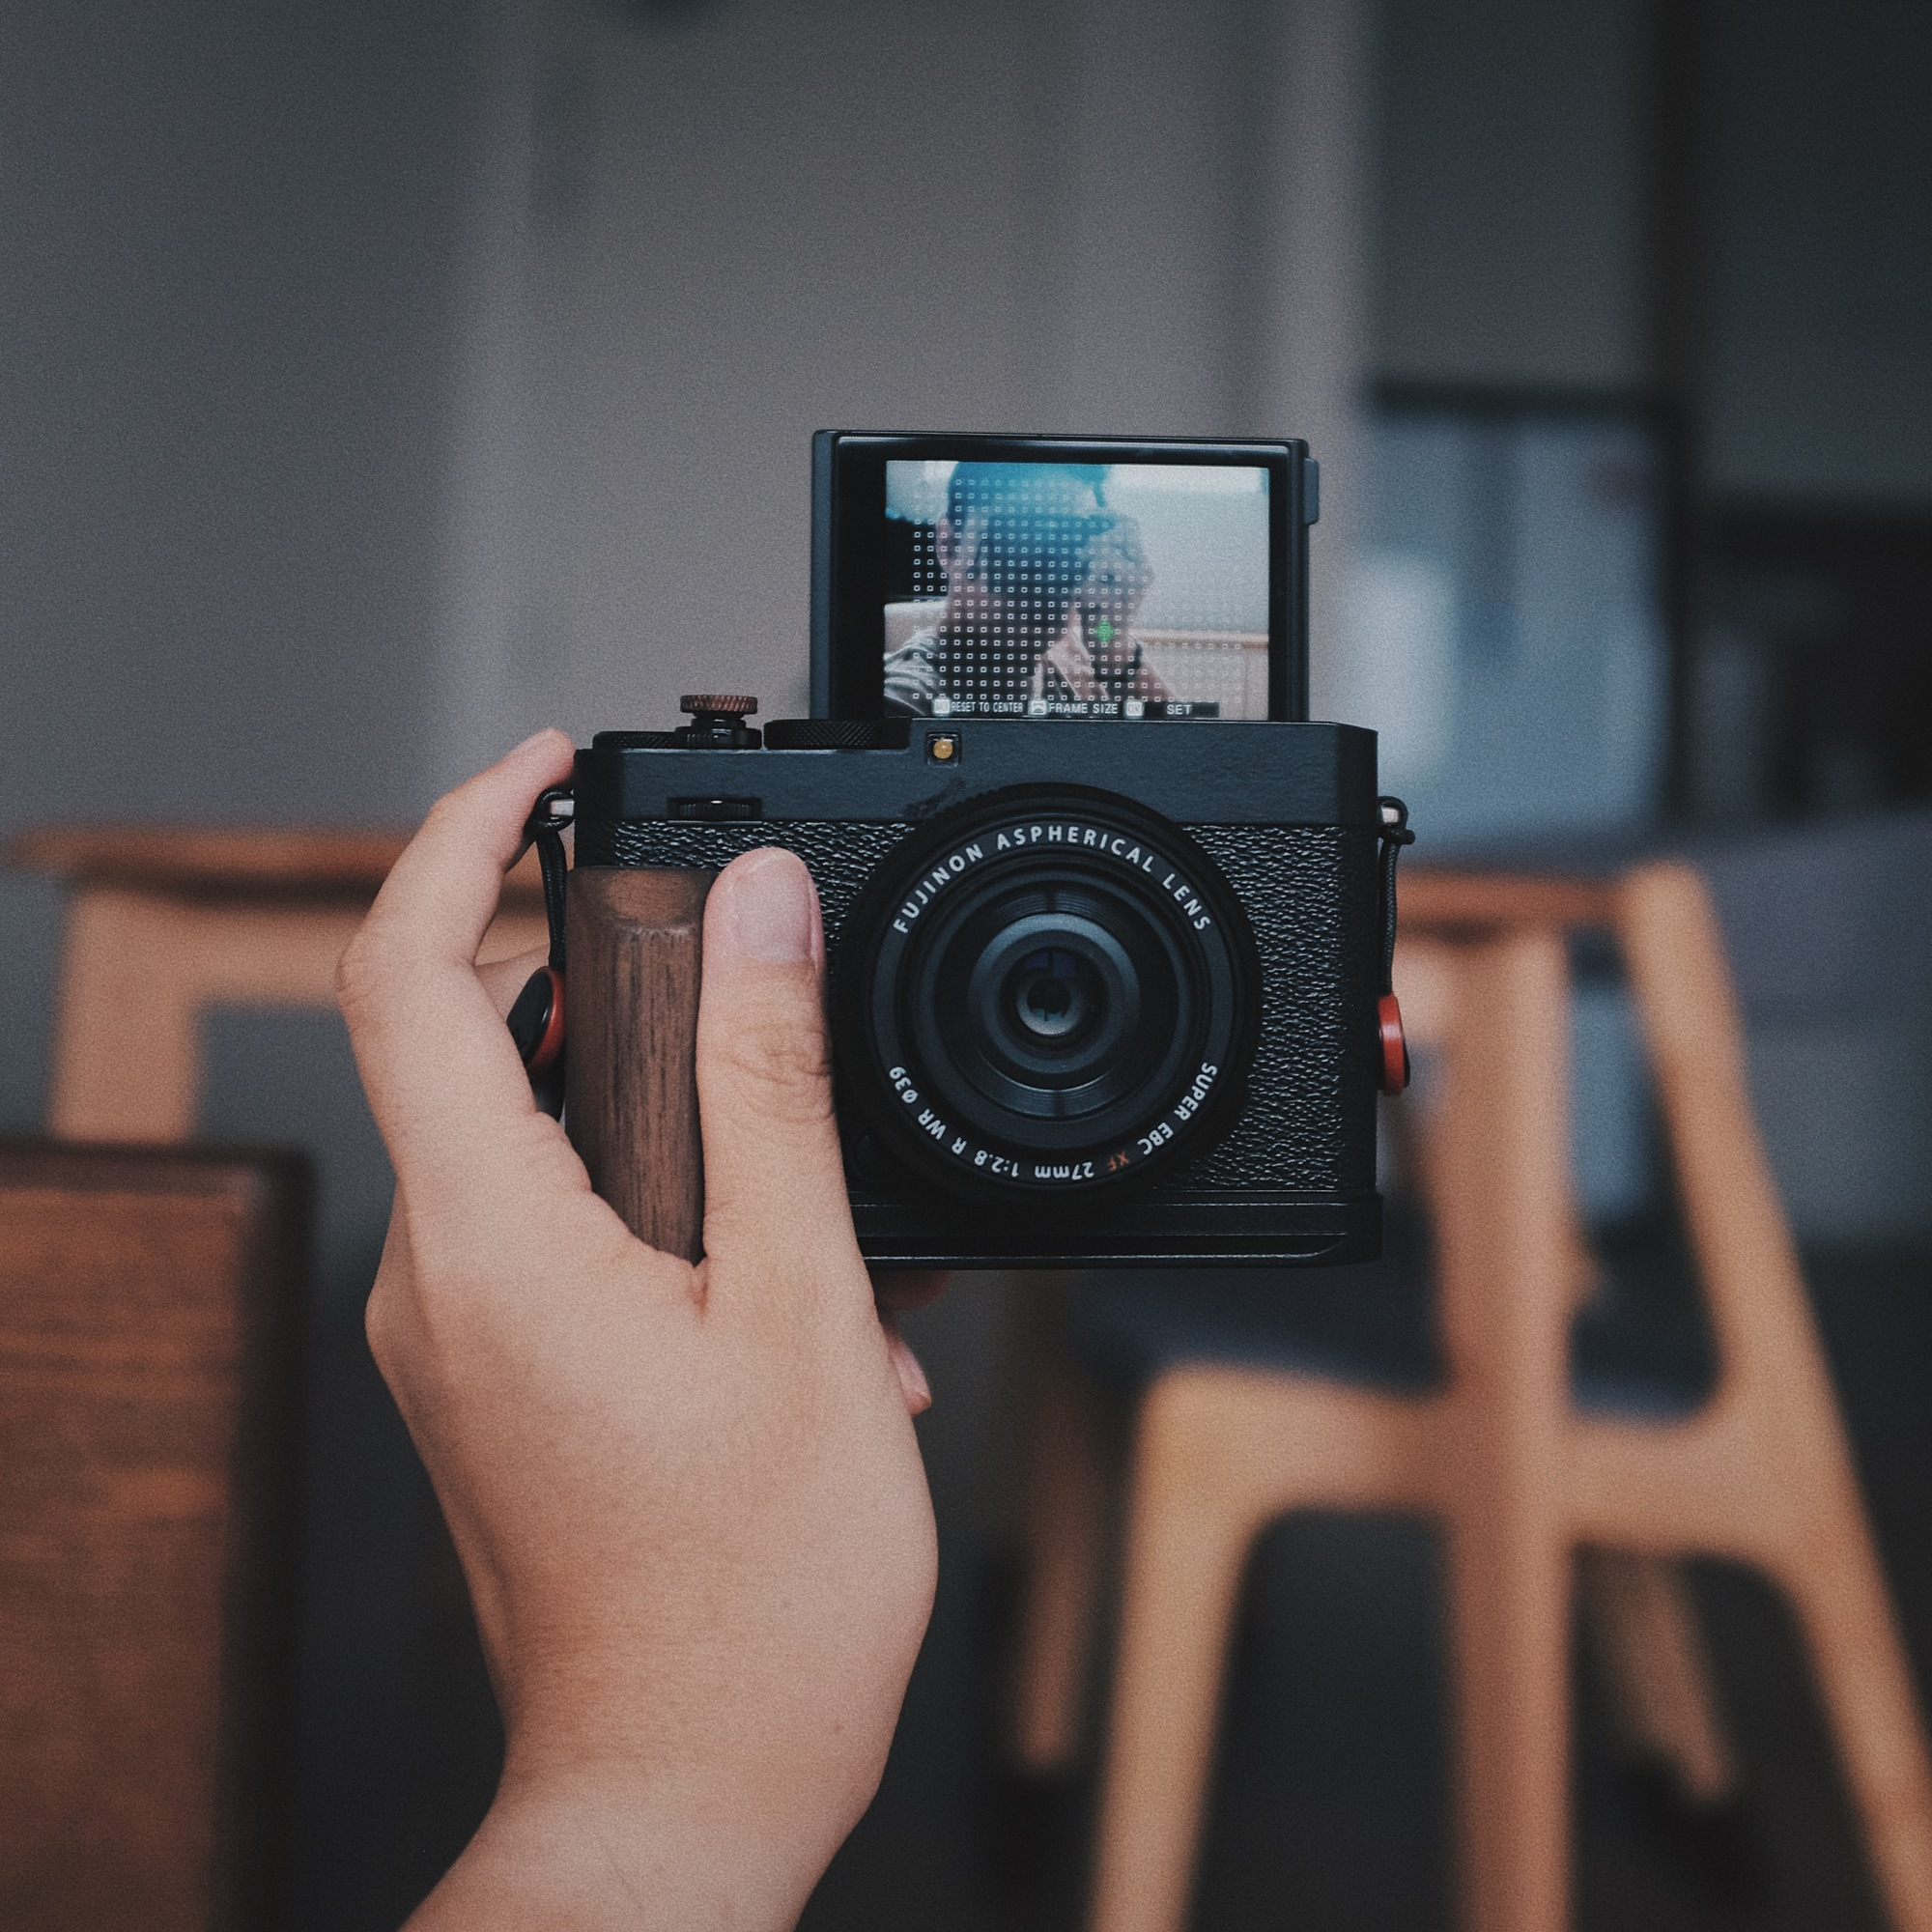
\includegraphics[width=\linewidth]{\envfinaldir/coverpic-prod.jpg}\par
            % \vskip 30pt
            \vfill

            \normalsize\rmfamily\scshape
            \copyright{} The Web Digest Project \hfill\large \envdatestr
        \end{center}
    \end{titlepage}
    % \restoregeometry
}
\newcommand{\simplehref}[1]{%
    \textcolor{blue!80!green}{\href{#1}{#1}}%
}
\renewcommand{\contentsname}{\center\Huge\sffamily\bfseries Contents\par\vskip 20pt}
\newcounter{ipartcounter}
\setcounter{ipartcounter}{0}
\newcommand{\ipart}[1]{
    % \vskip 20pt
    \clearpage
    \stepcounter{ipartcounter}
    \phantomsection
    \addcontentsline{toc}{chapter}{#1}
    % \begin{center}
    %     \Huge
    %     \sffamily\bfseries
    %     #1
    % \end{center}
    % \vskip 20pt plus 7pt
}
\newcounter{ichaptercounter}
\setcounter{ichaptercounter}{0}
\newcommand{\ichapter}[1]{
    % \vskip 20pt
    \clearpage
    \stepcounter{ichaptercounter}
    \phantomsection
    \addcontentsline{toc}{section}{\numberline{\arabic{ichaptercounter}}#1}
    \begin{center}
        \Huge
        \sffamily\bfseries
        #1
    \end{center}
    \vskip 20pt plus 7pt
}
\newcommand{\entrytitlefont}[1]{\subsection*{\raggedright\Large\sffamily\bfseries#1}}
\newcommand{\entryitemGeneric}[2]{
    % argv: title, url
    \parbox{\linewidth}{
        \entrytitlefont{#1}\par\vskip 5pt
        \footnotesize\ttfamily\mdseries
        \simplehref{#2}
    }\vskip 11pt plus 11pt minus 1pt
}
\newcommand{\entryitemGithub}[3]{
    % argv: title, url, desc
    \parbox{\linewidth}{
        \entrytitlefont{#1}\par\vskip 5pt
        \footnotesize\ttfamily\mdseries
        \simplehref{#2}\par\vskip 5pt
        \small\rmfamily\mdseries#3
    }\vskip 11pt plus 11pt minus 1pt
}
\newcommand{\entryitemAp}[3]{
    % argv: title, url, desc
    \parbox{\linewidth}{
        \entrytitlefont{#1}\par\vskip 5pt
        \footnotesize\ttfamily\mdseries
        \simplehref{#2}\par\vskip 5pt
        \small\rmfamily\mdseries#3
    }\vskip 11pt plus 11pt minus 1pt
}
\newcommand{\entryitemHackernews}[3]{
    % argv: title, hnurl, rawurl
    % \parbox{\linewidth}{
    %     \entrytitlefont{#1}\par\vskip 5pt
    %     \footnotesize\ttfamily\mdseries
    %     \simplehref{#3}\par
    %     \textcolor{black!50}{\href{#2}{#2}}
    % }\vskip 11pt plus 11pt minus 1pt
    \begin{minipage}{\linewidth}
            \entrytitlefont{#1}\par\vskip 5pt
            \footnotesize\ttfamily\mdseries
            \simplehref{#3}\par
            \textcolor{black!50}{\href{#2}{#2}}
    \end{minipage}\par\vskip 11pt plus 11pt minus 1pt
}







\begin{document}

\makeheader

\tableofcontents\clearpage




\ipart{Developers}
\ichapter{Hacker News}
\entryitemTwoLinks{Proton Mail suspended journalist accounts at request of cybersecurity agency}{https://news.ycombinator.com/item?id=45226903}{https://theintercept.com/2025/09/12/proton-mail-journalist-accounts-suspended/}

\entryitemTwoLinks{I used standard Emacs extension-points to extend org-mode}{https://news.ycombinator.com/item?id=45226639}{https://edoput.it/2025/04/16/emacs-paradigm-shift.html}

\entryitemTwoLinks{UTF-8 is a brilliant design}{https://news.ycombinator.com/item?id=45225098}{https://iamvishnu.com/posts/utf8-is-brilliant-design}

\entryitemTwoLinks{EU court rules nuclear energy is clean energy}{https://news.ycombinator.com/item?id=45224967}{https://www.weplanet.org/post/eu-court-rules-nuclear-energy-is-clean-energy}

\entryitemTwoLinks{Epistemic Collapse at the WSJ}{https://news.ycombinator.com/item?id=45224649}{https://www.math.columbia.edu/~woit/wordpress/?p=15206}

\entryitemTwoLinks{QGIS is a free, open-source, cross platform geographical information system}{https://news.ycombinator.com/item?id=45224156}{https://github.com/qgis/QGIS}

\entryitemTwoLinks{Corporations are trying to hide job openings from US citizens}{https://news.ycombinator.com/item?id=45223719}{https://thehill.com/opinion/finance/5498346-corporate-america-has-been-trying-to-hide-job-openings-now-it-is-failing/}

\entryitemTwoLinks{A beginner's guide to extending Emacs}{https://news.ycombinator.com/item?id=45223239}{https://blog.tjll.net/a-beginners-guide-to-extending-emacs/}

\entryitemTwoLinks{Crates.io phishing attempt}{https://news.ycombinator.com/item?id=45222772}{https://fasterthanli.me/articles/crates-io-phishing-attempt}

\entryitemTwoLinks{Many hard LeetCode problems are easy constraint problems}{https://news.ycombinator.com/item?id=45222695}{https://buttondown.com/hillelwayne/archive/many-hard-leetcode-problems-are-easy-constraint/}

\entryitemTwoLinks{3D modeling with paper}{https://news.ycombinator.com/item?id=45222369}{https://www.arvinpoddar.com/blog/3d-modeling-with-paper}

\entryitemTwoLinks{Ships are sailing with fake insurance from the Norwegian Ro Marine}{https://news.ycombinator.com/item?id=45221996}{https://www.nrk.no/vestland/xl/over-100-ships-have-sailed-without-legitimate-insurance-from-the-norwegian-company-ro-marine-1.17565216}

\entryitemTwoLinks{Chat Control faces blocking minority in the EU}{https://news.ycombinator.com/item?id=45221580}{https://twitter.com/TutaPrivacy/status/1966384776883142661}

\entryitemTwoLinks{The treasury is expanding the Patriot Act to attack Bitcoin self custody}{https://news.ycombinator.com/item?id=45221274}{https://www.tftc.io/treasury-iexpanding-patriot-act/}

\entryitemTwoLinks{Becoming the person who does the thing}{https://news.ycombinator.com/item?id=45220656}{https://www.fredrivett.com/2025/09/10/becoming-the-person-who-does-the-thing/}

\entryitemTwoLinks{Show HN: I made a generative online drum machine with ClojureScript}{https://news.ycombinator.com/item?id=45220069}{https://dopeloop.ai/beat-maker/}

\entryitemTwoLinks{Qwen3-Next}{https://news.ycombinator.com/item?id=45219228}{https://qwen.ai/blog?id=4074cca80393150c248e508aa62983f9cb7d27cd\&from=research.latest-advancements-list}

\entryitemTwoLinks{Debian 13, Postgres, and the US time zones}{https://news.ycombinator.com/item?id=45218111}{https://rachelbythebay.com/w/2025/09/11/debtz/}

\entryitemTwoLinks{The challenge of maintaining curl}{https://news.ycombinator.com/item?id=45217858}{https://lwn.net/Articles/1034966/}

\entryitemTwoLinks{The effects of algorithms on the public discourse}{https://news.ycombinator.com/item?id=45217545}{https://tekhne.dev/internet-resist/}\ichapter{Phoronix}
\entryitemGeneric{\hskip 0pt{}Wine 10.15 Released With Initial NTSYNC Bits, Unicode 17.0 Support}{https://www.phoronix.com/news/Wine-10.15-Released}

\entryitemGeneric{\hskip 0pt{}Intel i915 vs. Xe Graphics Driver Benchmarks For Meteor Lake: Extra Performance In 2025}{https://www.phoronix.com/review/intel-mtl-i915-xe-linux}

\entryitemGeneric{\hskip 0pt{}Intel Linux Graphics Driver Seeing 2~5\% Faster Shader Compilation Times, Up To ~20\%}{https://www.phoronix.com/news/Mesa-25.3-Faster-Intel-Shader}

\entryitemGeneric{\hskip 0pt{}Linux Mint 22.3 Planned To Bring More Wayland Improvements}{https://www.phoronix.com/news/Linux-Mint-22.3-Plans}

\entryitemGeneric{\hskip 0pt{}Fish Shell 4.0.6 Released With Many Fixes}{https://www.phoronix.com/news/Fish-Shell-4.0.6-Released}

\entryitemGeneric{\hskip 0pt{}Samba 4.23 Released With SMB3 Over QUIC, SMB3 Unix Extensions By Default}{https://www.phoronix.com/news/Samba-4.23-Released}

\entryitemGeneric{\hskip 0pt{}Linux 6.17 Fix Lands To Address Regression With "Serious Breakage" In Hibernation}{https://www.phoronix.com/news/Linux-6.17-PM-Hibernation-FIxes}

\entryitemGeneric{\hskip 0pt{}Fwupd 2.0.16 Released With New Search Feature, Fixes For FreeBSD Firmware Updates}{https://www.phoronix.com/news/Fwupd-2.0.16-Released}

\entryitemGeneric{\hskip 0pt{}Bcachefs Outlines Plans For Shipping As A DKMS Out-Of-Tree Kernel Module}{https://www.phoronix.com/news/Bcachefs-DKMS-Plans}


\ipart{Developers~~~~(zh-Hans)}
\ichapter{Solidot}
\entryitemGeneric{\hskip 0pt{}AirPods 实时翻译功能暂不向欧洲和中国大陆提供}{https://www.solidot.org/story?sid=82295}

\entryitemGeneric{\hskip 0pt{}全球消费的鳗鱼 99\% 属于濒危物种}{https://www.solidot.org/story?sid=82294}

\entryitemGeneric{\hskip 0pt{}矮行星鸟神星发现甲烷气体}{https://www.solidot.org/story?sid=82293}

\entryitemGeneric{\hskip 0pt{}章鱼有偏好使用的腕足}{https://www.solidot.org/story?sid=82292}

\entryitemGeneric{\hskip 0pt{}Windows 开发者可免费在 Microsoft Store 发布应用}{https://www.solidot.org/story?sid=82291}

\entryitemGeneric{\hskip 0pt{}Vimeo 以 13.8 亿美元出售给 Bending Spoons}{https://www.solidot.org/story?sid=82290}

\entryitemGeneric{\hskip 0pt{}Firefox 支持播放 MKV 内容}{https://www.solidot.org/story?sid=82289}

\entryitemGeneric{\hskip 0pt{}openSUSE 将禁用 bcachefs}{https://www.solidot.org/story?sid=82288}

\entryitemGeneric{\hskip 0pt{}NASA 禁止中国公民参与其太空项目}{https://www.solidot.org/story?sid=82287}

\entryitemGeneric{\hskip 0pt{}为什么 Netflix 难以制作出高质量电影}{https://www.solidot.org/story?sid=82286}

\entryitemGeneric{\hskip 0pt{}引力波证实霍金黑洞面积定理}{https://www.solidot.org/story?sid=82285}

\entryitemGeneric{\hskip 0pt{}法国配音演员指控《古墓丽影 4-6 重制版》使用 AI 合成其声音}{https://www.solidot.org/story?sid=82284}

\entryitemGeneric{\hskip 0pt{}小红书被要求限期整改}{https://www.solidot.org/story?sid=82283}

\entryitemGeneric{\hskip 0pt{}甲骨文股价飙升,Larry Ellison 成为新首富}{https://www.solidot.org/story?sid=82282}

\entryitemGeneric{\hskip 0pt{}研究发现爱喝啤酒的人对蚊子有高吸引力}{https://www.solidot.org/story?sid=82281}

\entryitemGeneric{\hskip 0pt{}NASA 称毅力号漫游车在火星发现潜在生物特征}{https://www.solidot.org/story?sid=82280}

\entryitemGeneric{\hskip 0pt{}疫情期间使用的一次性口罩留下了化学定时炸弹}{https://www.solidot.org/story?sid=82279}

\entryitemGeneric{\hskip 0pt{}婴儿的哭泣声会让人的身体发热}{https://www.solidot.org/story?sid=82278}

\entryitemGeneric{\hskip 0pt{}Windows 10 拒绝消失}{https://www.solidot.org/story?sid=82277}

\entryitemGeneric{\hskip 0pt{}更温暖的气候可能会增加添加糖摄入量}{https://www.solidot.org/story?sid=82276}\ichapter{V2EX}
\entryitemGeneric{\hskip 0pt{}[生活] 10 年前的 10 万元相当于现在多少钱?}{https://www.v2ex.com/t/1158917}

\entryitemGeneric{\hskip 0pt{}[分享创造] Neuralrad Mammo V2.1 更新免费帮助用户分析乳腺钼靶图像的 AI 工具}{https://www.v2ex.com/t/1158915}

\entryitemGeneric{\hskip 0pt{}[生活方式] 说真的,买套房把父母接过来过一辈子事实也挺好的}{https://www.v2ex.com/t/1158914}

\entryitemGeneric{\hskip 0pt{}[分享创造] [娱乐向] Vibe 了一个游戏策划,包含设定,故事等等,名称叫 『几何境域:形态之战』希望能做个 Demo 出来}{https://www.v2ex.com/t/1158912}

\entryitemGeneric{\hskip 0pt{}[iPhone] iPhone 17 v 友们选了哪个型号下单?}{https://www.v2ex.com/t/1158911}

\entryitemGeneric{\hskip 0pt{}[分享创造] 分享一个自用的 [LeetCode HOT 100] 刷题模版}{https://www.v2ex.com/t/1158910}

\entryitemGeneric{\hskip 0pt{}[程序员] 毕业一年,想 9 月中下旬请个小长假+国庆冲刺金九银十}{https://www.v2ex.com/t/1158909}

\entryitemGeneric{\hskip 0pt{}[分享创造] cascade - 自动从代办事项生成日程计划}{https://www.v2ex.com/t/1158908}

\entryitemGeneric{\hskip 0pt{}[问与答] 小红书要被查什么?}{https://www.v2ex.com/t/1158905}

\entryitemGeneric{\hskip 0pt{}[阅读] 2025 八月读自由主义 魔法 蘑菇 ADHD AI … 10 本}{https://www.v2ex.com/t/1158904}

\entryitemGeneric{\hskip 0pt{}[投资] 币安合约跟单,虽然不多,但是一天一顿猪脚饭还是有的}{https://www.v2ex.com/t/1158903}

\entryitemGeneric{\hskip 0pt{}[Apple] 外版 esim 的 iPhone 不是支持国内运营商的 esim 吗?}{https://www.v2ex.com/t/1158901}

\entryitemGeneric{\hskip 0pt{}[生活] 扯什么预制菜的国家标准都没用}{https://www.v2ex.com/t/1158900}

\entryitemGeneric{\hskip 0pt{}[跑步] 赤脚参赛半马 成绩 1:29:30}{https://www.v2ex.com/t/1158899}

\entryitemGeneric{\hskip 0pt{}[日本] 可以在国内用的日本号码}{https://www.v2ex.com/t/1158898}

\entryitemGeneric{\hskip 0pt{}[分享发现] 罗永浩这次赢定!}{https://www.v2ex.com/t/1158897}

\entryitemGeneric{\hskip 0pt{}[Apple] 最新版 macOS 26 成功在国内连接 6Ghz WiFi}{https://www.v2ex.com/t/1158895}

\entryitemGeneric{\hskip 0pt{}[分享创造] 肝了一周,把 Nano Banana 画图的网站优化了一下}{https://www.v2ex.com/t/1158894}

\entryitemGeneric{\hskip 0pt{}[iPhone] Phone 17 Pro 中国内地版将独家采用京东方显示屏}{https://www.v2ex.com/t/1158893}

\entryitemGeneric{\hskip 0pt{}[分享创造] 我与 Gemini 深度协作编码的「提示词」(以及配套小工具)}{https://www.v2ex.com/t/1158892}

\entryitemGeneric{\hskip 0pt{}[推广] 即梦 Seadream 4.0 真比 NanoBanana 更好用?说说我的这几天真实体验}{https://www.v2ex.com/t/1158891}

\entryitemGeneric{\hskip 0pt{}[问与答] 校园宽带限制破解}{https://www.v2ex.com/t/1158890}

\entryitemGeneric{\hskip 0pt{}[分享发现] 即梦 4.0 限免 7 天,还有人不知道吗?}{https://www.v2ex.com/t/1158889}

\entryitemGeneric{\hskip 0pt{}[微信] 微信 PC 版小程序能否使用定位功能?}{https://www.v2ex.com/t/1158888}

\entryitemGeneric{\hskip 0pt{}[生活] 格力 ai 节能王子比同 apf 值的格力空调真的能省电 13\%吗}{https://www.v2ex.com/t/1158886}

\entryitemGeneric{\hskip 0pt{}[iPhone] 天猫国补+以旧换新下单 iPhone 17,一共¥ 4714}{https://www.v2ex.com/t/1158884}

\entryitemGeneric{\hskip 0pt{}[微信] 我的微信非常卡顿}{https://www.v2ex.com/t/1158882}

\entryitemGeneric{\hskip 0pt{}[iPhone] 抢到了 iPhone 17 Pro Max 2T}{https://www.v2ex.com/t/1158881}

\entryitemGeneric{\hskip 0pt{}[Apple] 有在天猫官旗下单的朋友吗?}{https://www.v2ex.com/t/1158880}

\entryitemGeneric{\hskip 0pt{}[iPhone] 天猫官网买的你们都是几天内发货?}{https://www.v2ex.com/t/1158879}

\entryitemGeneric{\hskip 0pt{}[Solana] 我去, 刚才使用 brave 打开 gmgn, 给我弹了个请求剪贴板权限, 给我惊了一下, 最近的盗币新闻太吓人了.}{https://www.v2ex.com/t/1158878}

\entryitemGeneric{\hskip 0pt{}[上海] 上海不是说没国补了么,要摇号,怎么一点就有?}{https://www.v2ex.com/t/1158877}

\entryitemGeneric{\hskip 0pt{}[分享创造] 我是名面临被裁的土木从业者自学 2 个月做出人生第一个在线图片转换工具站}{https://www.v2ex.com/t/1158876}

\entryitemGeneric{\hskip 0pt{}[Apple] 苹果官网和 Apple Store App 送货时间是在下单前确定还是下单后确定的?}{https://www.v2ex.com/t/1158875}

\entryitemGeneric{\hskip 0pt{}[iPhone] 港版备货充足}{https://www.v2ex.com/t/1158874}

\entryitemGeneric{\hskip 0pt{}[iPhone] 首发官网已冲}{https://www.v2ex.com/t/1158872}

\entryitemGeneric{\hskip 0pt{}[宽带症候群] 成都电信高峰期卡顿}{https://www.v2ex.com/t/1158871}

\entryitemGeneric{\hskip 0pt{}[iPhone] iPhone Air 现在不让买。。。无语}{https://www.v2ex.com/t/1158870}

\entryitemGeneric{\hskip 0pt{}[Apple] 你们买得到 iPhone17 吗?天猫狗东我都看不到有货的页面就没有了,无论颜色还是容量,全部卖光,什么情况?}{https://www.v2ex.com/t/1158869}

\entryitemGeneric{\hskip 0pt{}[加密货币] 关于出入金是否会涉及到非法换汇}{https://www.v2ex.com/t/1158868}

\entryitemGeneric{\hskip 0pt{}[iPhone] ios 本机如何安装已签名的 ipa?}{https://www.v2ex.com/t/1158866}

\entryitemGeneric{\hskip 0pt{}[Apple] iPhone17 多多补贴 200 元, 5799 起}{https://www.v2ex.com/t/1158865}

\entryitemGeneric{\hskip 0pt{}[分享创造] 🎵 [送码] Audio Editor(音频工具箱)- 全能音频处理神器,限时免费兑换 PRO 终身版!}{https://www.v2ex.com/t/1158864}

\entryitemGeneric{\hskip 0pt{}[Apple] 苹果 cn 官网的订单状态查阅服务是被人为关闭了还是自己炸了啊?}{https://www.v2ex.com/t/1158863}

\entryitemGeneric{\hskip 0pt{}[Apple] Apple Intelligence 的多模态模型 AFM 能开放出来支持 cURL 的 local server 吗?}{https://www.v2ex.com/t/1158862}

\entryitemGeneric{\hskip 0pt{}[V2EX] 🎵 [新品发布] Audio Editor(音频工具箱)- 全能音频处理神器,限时免费兑换 PRO 终身版!}{https://www.v2ex.com/t/1158861}

\entryitemGeneric{\hskip 0pt{}[推广] 20.5 元吃紫光园|奶皮子酸奶,爱吃的有福了,可配送可自提}{https://www.v2ex.com/t/1158860}

\entryitemGeneric{\hskip 0pt{}[Apple] 你的城市 iPhone 17 和 17 Pro 真机线下直营店可以上手体验了吗?}{https://www.v2ex.com/t/1158858}

\entryitemGeneric{\hskip 0pt{}[iPhone] 17pro 512g 双十一是否应该抢首发?}{https://www.v2ex.com/t/1158857}

\entryitemGeneric{\hskip 0pt{}[数据库] 有个关于 mongodb 的问题,求大神来解答一下}{https://www.v2ex.com/t/1158855}


\ipart{Generic News}







\clearpage
\leavevmode\vfill
\footnotesize

Copyright \copyright{} 2023-2025 Neruthes and other contributors.

This document is published with CC BY-NC-ND 4.0 license.

The entries listed in this newsletter may be copyrighted by their respective creators.

This newsletter is generated by the Web Digest project.

The newsletters are also delivered via Telegram channel \CJKunderline{\href{https://t.me/webdigestchannel}{https://t.me/webdigestchannel}}.\\
RSS feed is available at \CJKunderline{\href{https://webdigest.pages.dev/rss.xml}{https://webdigest.pages.dev/rss.xml}}.

This newsletter is available in PDF at
\CJKunderline{\href{https://webdigest.pages.dev/}{https://webdigest.pages.dev/}}.

The source code being used to generate this newsletter is available at\\
\CJKunderline{\href{https://github.com/neruthes/webdigest}{https://github.com/neruthes/webdigest}}.

This newsletter is also available in
\CJKunderline{\href{http://webdigest.pages.dev/readhtml/\envyear/WebDigest-20250913.html}{HTML}} and
\CJKunderline{\href{https://github.com/neruthes/webdigest/blob/master/markdown/\envyear/WebDigest-20250913.md}{Markdown}}.


\coverpic{https://unsplash.com/photos/a-black-and-white-photo-of-a-computer-keyboard-muvgkVuKPDo}{Pawel Czerwinski}


\end{document}
